\section{Intro to random sampling}

The \href{https://github.com/libmir/mir/pull/240}{code} is currently \textcolor{red}{WIP} and will be available at \texttt{mir.random.flex}. The report \textit{Transformed Density Rejection with Inflection Points} can be found  \href{http://epub.wu.ac.at/3158/1/techreport-110.pdf}{here}.

\subsection{WIP}

If you have ideas how to improve this report, shoot them at me (seb@wilzba.ch).
All code listings can be browsed online at \url{https://github.com/wilzbach/flex-paper}.

\subsection{The problem}

Given a uniform random generator, sample \textit{non-uniform random} values.

The following subsections will introduce some of the basi methods of the
random sampling, which are also used by the Flex algorithm.

\subsection{The inversion method}
\label{subsection:inversion}

The underlying idea of random sampling is that given an inverse function $F^{-1}$ for the cumulative density function (CDF) of a target density $f(x)$, random values can be mapped to a distribution. Given $F^{-1}$ values from the density can be sampled by using the given uniform random generator (of the interval $[0, 1]$).
For example, for the exponential distribution sampling would be:

\begin{lstlisting}[language=D]
S sample(S, RNG, FInv)(RNG gen, FInv finv)
{
    import std.random : uniform;
    S u = uniform!("[]", S)(0, 1);
    return finv(u);
}
import std.random : rndGen;
auto fInvExp = (S x) => -log(S(1) - x);
sample(rndGen, fInvExp)
\end{lstlisting}

More visually you can imagine this with the cumulative plot at \autoref{fig:expo_inv}.
We randomly pick a point $y$ on the CDF graph and then use the \textit{inverse}
function to get the matching value $x$, e.g. if we sample $0.4$ (brown line) the algorithm
would return $-log(1 - 0.4) = 0.51$, for $0.6$ (yellow) it would be $0.91$ and for
$0.9$ (yellow) it would be $2.30$ respectively.

\begin{figure}
    \centering
    \begin{subfigure}[b]{0.49\textwidth}
        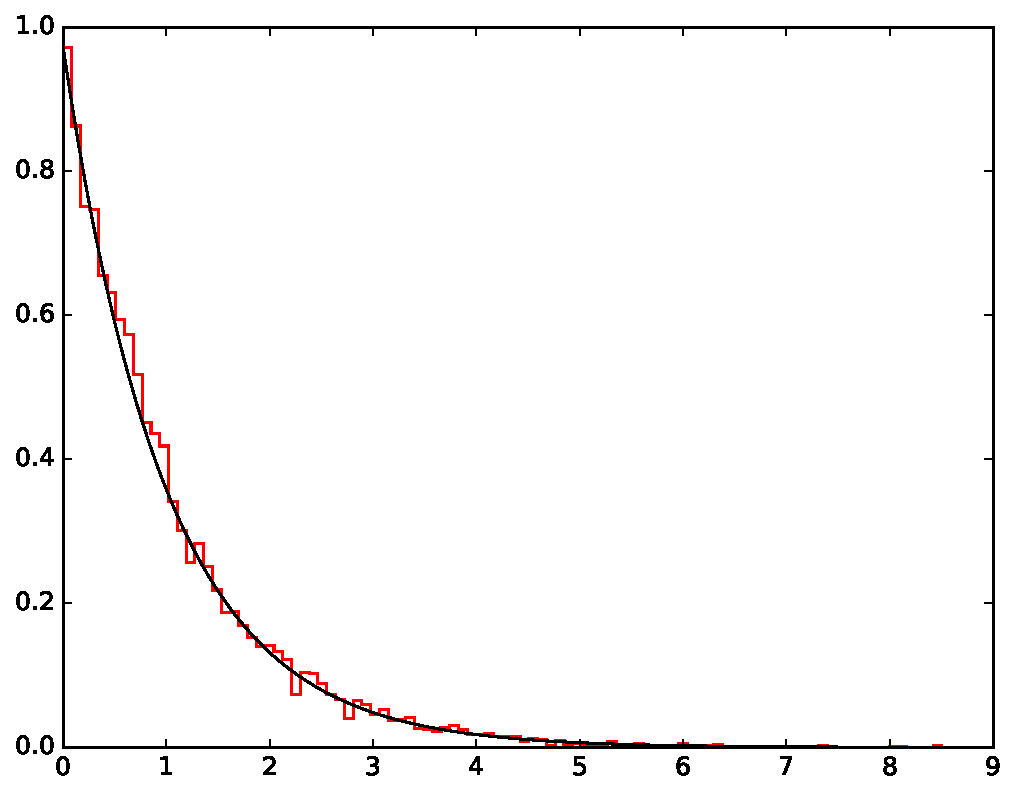
\includegraphics[width=\textwidth]{figs/expo.pdf}
        \caption{Exponential distribution}
    \end{subfigure}
    \begin{subfigure}[b]{0.49\textwidth}
        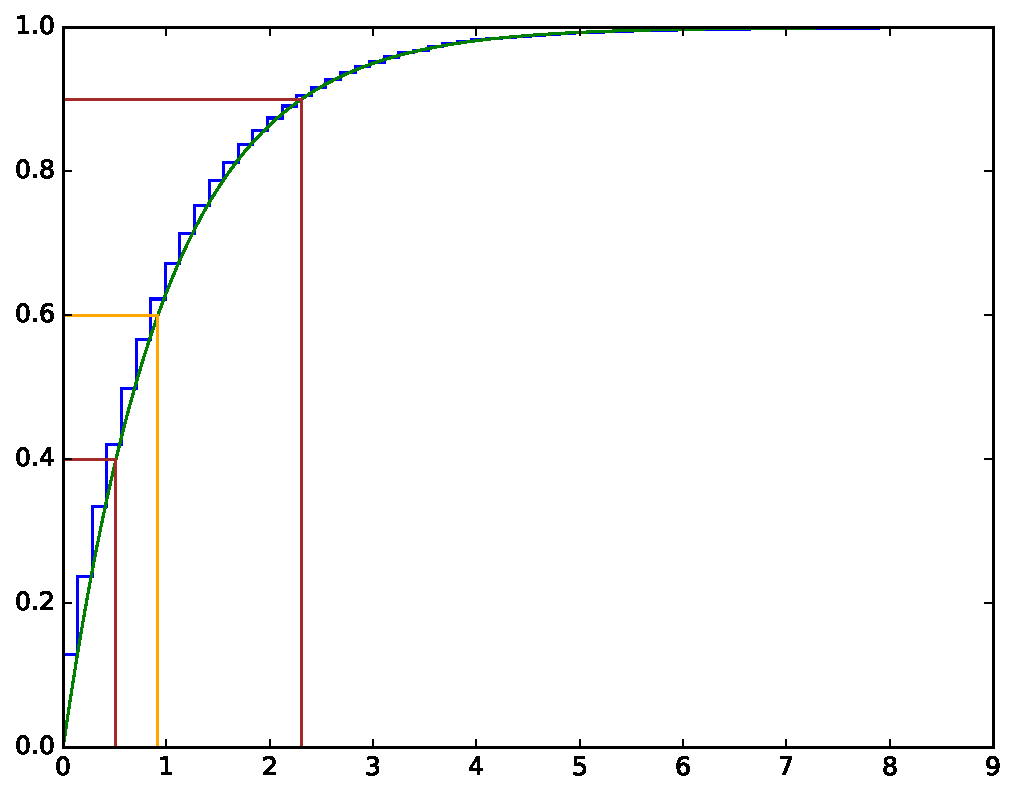
\includegraphics[width=\textwidth]{figs/inversion_sampling.pdf}
        \caption{Exponential distribution, cumlative}
    \end{subfigure}
    \caption{Sampling from the exponential distribution using the inversion method.}
     \label{fig:expo_inv}
\end{figure}

However there are two big problems of the inversion method: (1) for most densities the inverse CDF is not known or can't be determined or (2) if it can be determined it's usually very computationally expensive function (e.g. iterative numeric approximation needs to be used if no exact form can be found).

\subsection{The rejection method}
\label{subsection:rejection}

A very popular alternative is the \textit{rejection} method - often known as \textit{acceptance-rejection} sampling. It only requires one to know the density of a distribution. The general idea is that if a random variable $(x, y)$ is distributed within the density $f$, then it has the density $f$ (blue in \autoref{fig:rejection_method}).

This means we can sample $x$ and $y$ uniformly within the area that is strictly larger than $f$ and check whether the generated point is in the area covered by the density function. If it's within the area the point is \textit{accepted} (black in \autoref{fig:rejection_method}), otherwise it is \textit{rejected} (brown in \autoref{fig:rejection_method})) and new points are sampled until a point, which is within the area and thus can be accepted, is drawn.

More formally, a hat function $h(x)$ that majorizes the density function $f(x)$ is needed. In other words $ \forall x \in [l, r]: f(x) < h(x)$, where $l$ and $r$ are the left and right boundaries of an interval.
The hat function (green in \autoref{fig:rejection_method}) is the boundary function for our target density sampling. In this simple example the hat function would be the horizontal line $x = 1$.

\begin{figure}[h!]
\centering
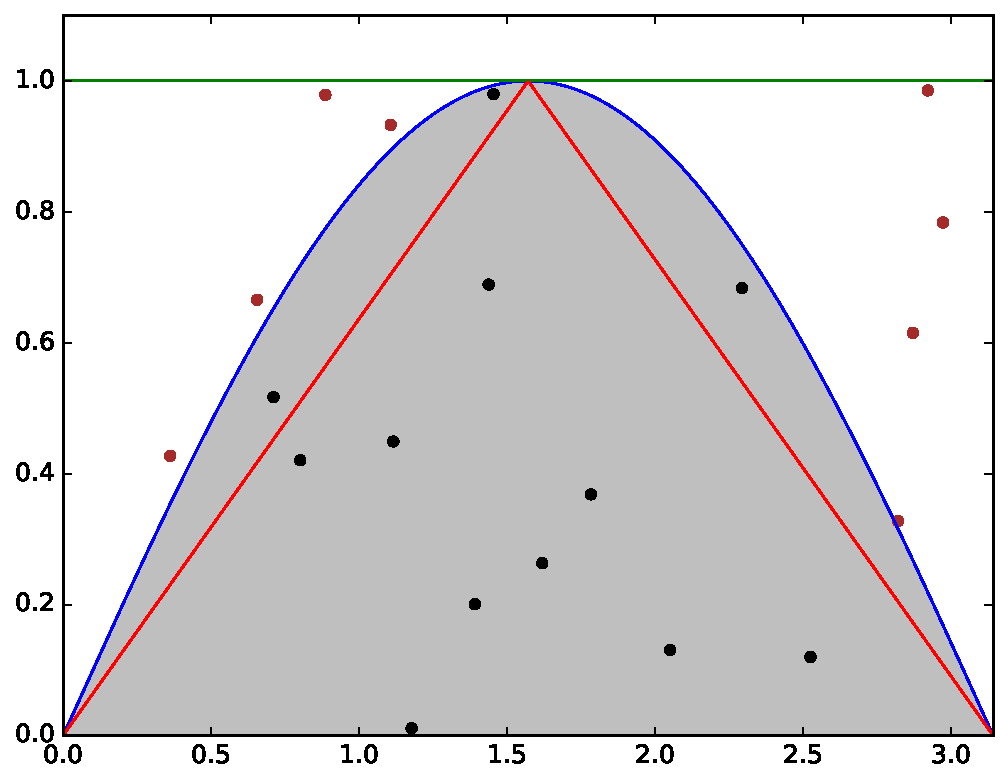
\includegraphics[width=0.8\textwidth]{figs/rejection_sampling.pdf}
\caption{Rejection sampling of $sin(x)$ (blue). Hat function ($x = 1$) is drawn in green, whereas the squeeze function ($1 - |1 - 2x / \pi |$) is drawn in red. Points are marked black when accepted, and brown for rejected.}
\label{fig:rejection_method}
\end{figure}

It is important to see that for every point $x$ we evaluate whether it's within the density area $f(x)$. As $h(x)$ is by definition always larger than $f(x)$ we can use $y * h(x) \leq f(x)$ when we want to programmatically check whether a generated point is within the target density as it covers the entire density of $f(x)$ (as $f(x) \in [0, 1]\  \forall x \in [\ell, r],\  y \in [0, 1]$)

A simplified example of the basic rejection method can be seen here:

\begin{minipage}{\linewidth}
\begin{lstlisting}[language=D]
S sample(RNG, Pdf, Hat, S)(ref RNG gen, Pdf pdf, Hat hat, S left, S right)
{
    import std.random : uniform;
    for (;;)
    {
        // generate x with density proportional to hat(x)
        S x = uniform!("[]", S)(left, right, gen);
        // generate "vertical" variable y to evaluate x
        S y = uniform!("[]", S)(0, 1, gen);
        // check whether the sampled point is within the density
        if (y * hat(x) <= pdf(x))
            return x;
    }
}
alias S = double;
import std.math : PI, sin;
import std.random: rndGen;
auto pdf = (S) => sin(x);
auto hat = (S x) => 1;
sample(rndGen, pdf, hat, S(0), PI);
\end{lstlisting}
\end{minipage}

Furthermore the performance of this method depends heavily on the ratio of $f(x) / h(x) = \alpha$, where $1 / \alpha$ is the average number of needed iterations to sample one value.

\subsection{Rejection with inversion}
\label{subsection:rejection_inversion}

Just a straight line as upper bound yields a lot of uncovered areas, thus a more generic \textit{hat} functions is necessary.
If the inverse of the \textit{hat} function is known, the inversion method can be used to sample from an arbitrary \textit{hat} function:

\begin{minipage}{0.9\linewidth}
\begin{lstlisting}[language=D]
S sample(S, RNG, Pdf, Hat, HatInv)(ref RNG gen, Pdf pdf, Hat hat,
                                       HatInv hatInvCDF)
{
    import std.random : uniform;
    for (;;)
    {
        // generate x with density proportional to hat(x)
        S u = uniform!("[]", S)(0, 1, gen);

		// map u uniquely to a point of the integral of hat(x)
        S x = hatInvCDF(u);

        // generate "vertical" variable y to evaluate x
        S y = uniform!("[]", S)(0, 1, gen);

        // check whether the sampled point is within the density
        if (y * hat(x) <= pdf(x))
            return x;
    }
}
import std.math : PI, sin;
import std.random: rndGen;
alias S = double;
auto pdf = (S) => sin(x);
auto hatInvCDF = (S u) => 0 + u * (PI - 0);
auto hat = (S x) => 1;
sample!S(rndGen, pdf, hat, hatInvCDF);
\end{lstlisting}
\end{minipage}

The (Tin)flex algorithm will show a way to automatically construct a hat function for any differentiable density function.

\subsection{Squeeze functions}
\label{subsection:squeeze}

Calculating the probability density function is often expensive, thus defining a lower bound that can evaluated much faster would be yield a performance boost.
This lower bound is called $s(x)$ which is majorized by $f(x)$, i.e. $s(x) \leq f(x) \forall x \in [l, r]$.
For example, the squeeze function in \autoref{fig:rejection_method} is $1 - |1 - 2x / \pi |$. If $x$ is below the squeeze function, it can be accepted \textit{without} the need to calculate the density function as by definition every point in the squeeze function $s(x)$ is also below $f(x)$. Hence the \textit{sample} routine can be adapted:

\begin{minipage}{0.9\linewidth}
\begin{lstlisting}[language=D]
S sample(S, RNG, Pdf, Hat, HatInv, Squeeze)(ref RNG gen, Pdf pdf,
                              Hat hat, HatInv hatInvCDF, Squeeze sq)
{
    import std.random : uniform;
    for (;;)
    {
        // generate x with density proportional to hat(x)
        S u = uniform!("[]", S)(0, 1, gen);
		// map u uniquely to a point of the integral of hat(x)
        S x = hatInvCDF(u);

        // generate "vertical" variable y to evaluate x
        S y = uniform!("[]", S)(0, 1, gen);
        S t = y * hat(x);

        // check whether the sampled point is below the squeeze
        if (t <= sq(x))
            return x;

        // check whether the sampled point is within the density
        if (y * hat(x) <= pdf(x))
            return x;
    }
}

import std.math : abs, PI, sin;
import std.random: rndGen;
alias S = double;
auto hatInvCDF = (S u) => 0 + u * (PI - 0);
auto hat = (S x) => 1;
auto sq = (S x) => 1 - abs(1 - 2 * x / PI);
sample!S(rndGen, (S) => sin(x), hat, hatInvCDF, sq);
\end{lstlisting}
\end{minipage}


\subsection{Composition}
\label{subsection:composition}

A density function might be split into multiple parts with each having it's own hat and squeeze.
If we are given multiple densities, we can sample from the overall density by picking from each sampler according to a given probability $p_i$ which is defined by their hat area.
For example, \autoref{fig:dist_composition} shows a distribution that is composed out of multiple hat and squeeze parts.

\begin{figure}[h!]
\centering
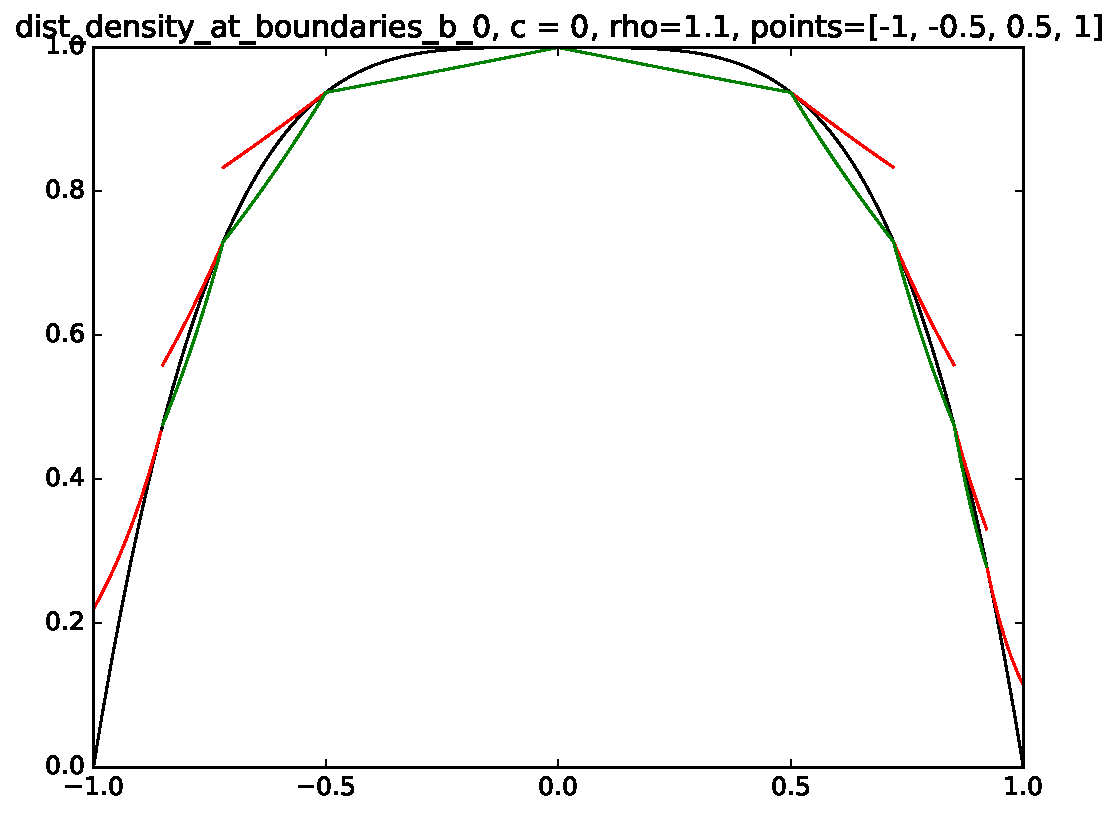
\includegraphics[width=0.8\textwidth]{figs/dist_density_at_boundaries_b_0_hs.pdf}
\caption{Distribution split into multiple hat (red) and squeeze (green) functions.}
\label{fig:dist_composition}
\end{figure}

The idea of composing distributions will be illustrated as follows.
The density function is composed out of an exponential distribution (left) and a uniform distribution (right) and features a gap in the middle.

\pagebreak

%\begin{minipage}{0.9\linewidth}
\begin{lstlisting}[language=D]
S sample(S, RNG, Sampler)(ref RNG gen, Sampler[] samplers, S[] probs)
{
    import mir.random.discrete : discrete;
    // pick a sampler with prob_i
    auto ds = discrete(probs);
    // sample with the chosen sampler
    return samplers[ds(gen)](gen);
}

import std.random: Mt19937, uniform, rndGen;
alias S = double;

alias Sampler = S delegate(ref typeof(gen) gen);
S[] probs = [0.7, 0.3];
Sampler[] samplers = new Sampler[probs.length];

// a part of the exponential distribution on the left
samplers[0] = (ref typeof (gen) gen) {
    import std.math : log;
    auto finv = (S x) => -log(S(1) - x);
    S u = uniform!("[)", S)(0, 0.8);
    return finv(u);
};

// a uniform sampler on the right half
samplers[1] = (ref typeof (gen) gen) {
    return uniform!("[]", S)(2, 3, gen);
};
sample!S(gen, samplers, probs);
\end{lstlisting}
%\end{minipage}

\ \\

The result of our basic composition with different target probabilities for the samples can be seen in \autoref{fig:composition_exp_uniform}. The (Tin)flex algorithm will automatically generate intervals with hat and squeeze function for the desired distribution that are connected with such a composition sampler.

\begin{figure}[h]
    \centering
    \begin{subfigure}[b]{0.49\textwidth}
        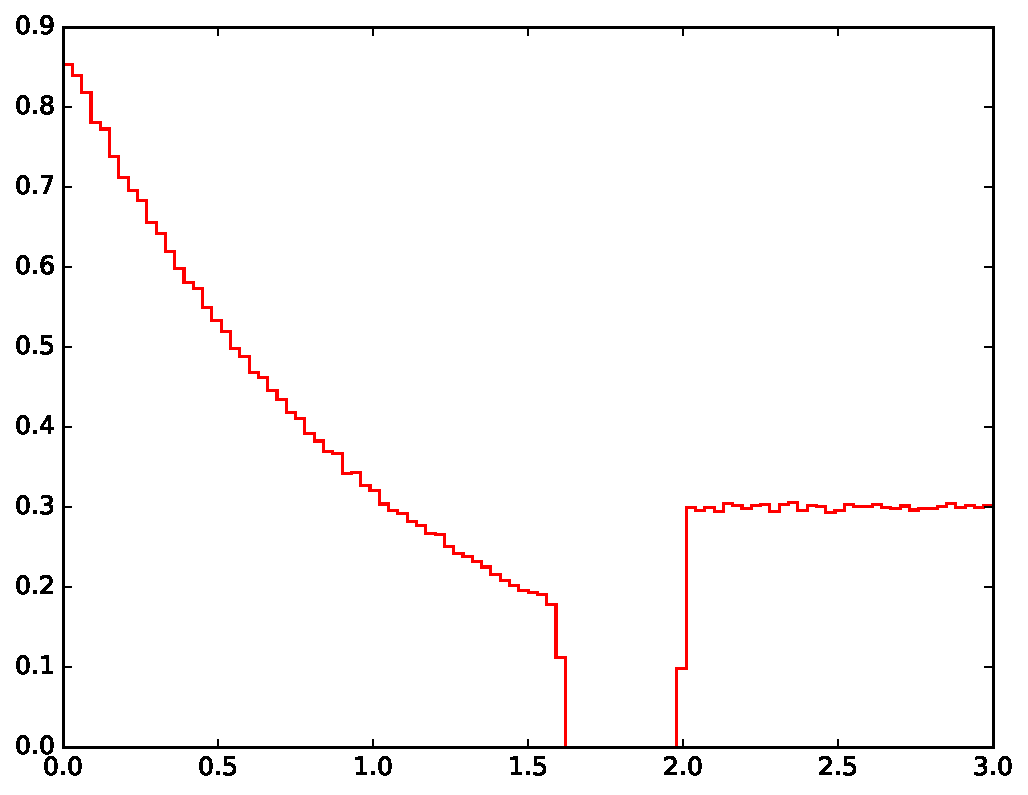
\includegraphics[width=\textwidth]{figs/composed_dist_70_30.pdf}
        \caption{$p = [0.7, 0.3]$}
    \end{subfigure}
    \begin{subfigure}[b]{0.49\textwidth}
        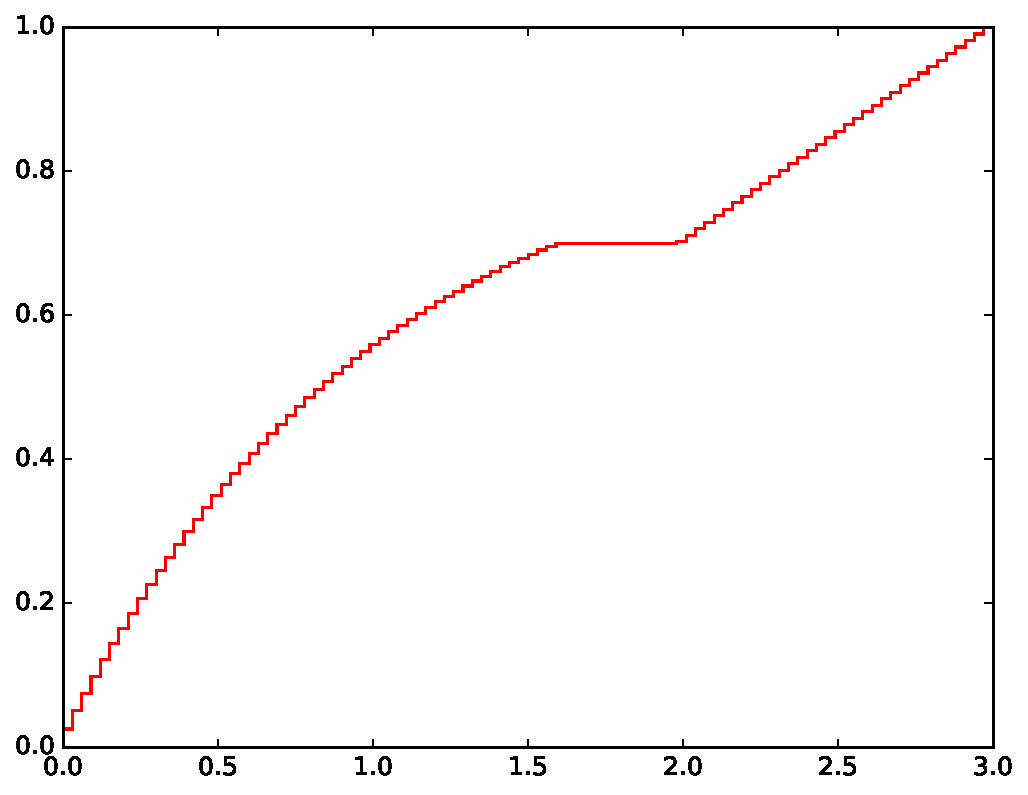
\includegraphics[width=\textwidth]{figs/composed_dist_70_30_cum.pdf}
        \caption{$p = [0.7, 0.3]$, cumlative}
    \end{subfigure}
    \centering
    \begin{subfigure}[b]{0.49\textwidth}
        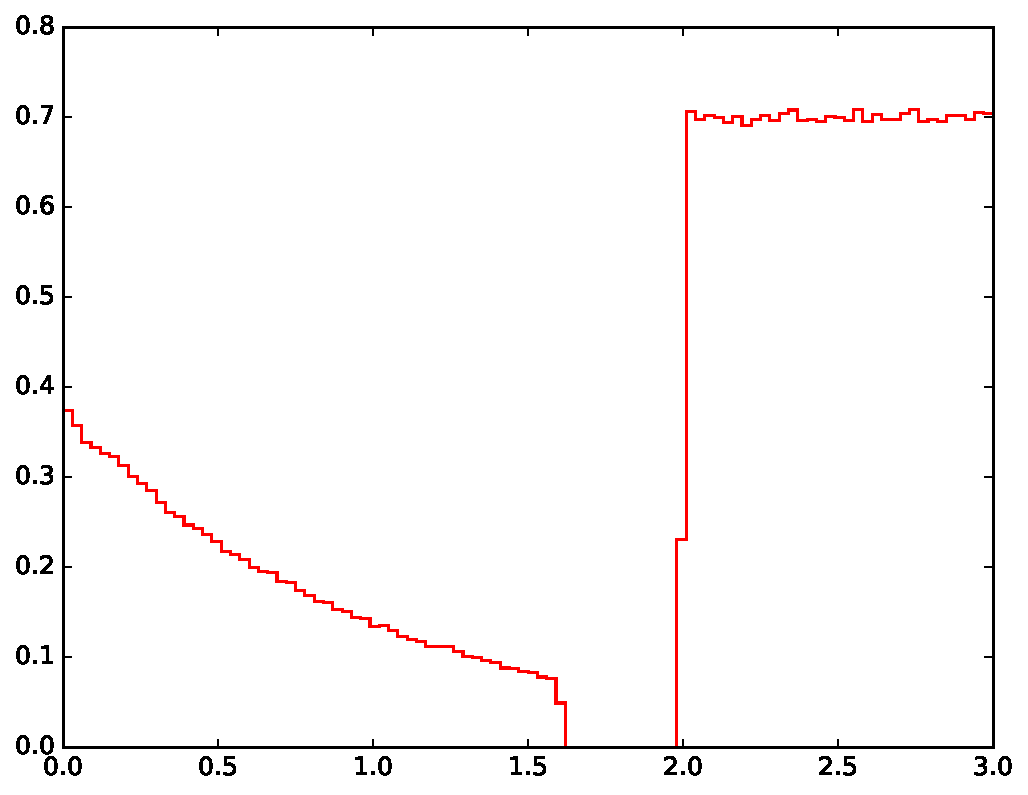
\includegraphics[width=\textwidth]{figs/composed_dist_30_70.pdf}
        \caption{$p = [0.3, 0.7]$}
    \end{subfigure}
    \begin{subfigure}[b]{0.49\textwidth}
        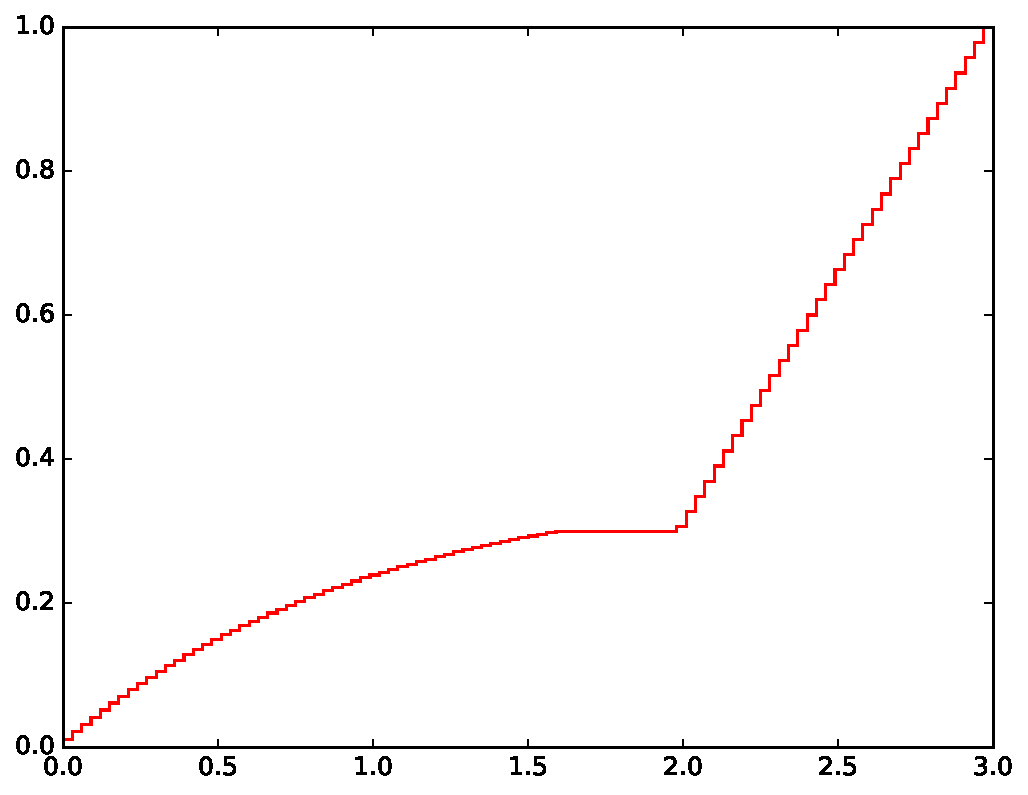
\includegraphics[width=\textwidth]{figs/composed_dist_30_70_cum.pdf}
        \caption{$p = [0.3, 0.7]$, cumulative}
    \end{subfigure}
    \caption{Composition of exponential and uniform distribution}
     \label{fig:composition_exp_uniform}
\end{figure}


